%%%%%%%%%%%%%%%%%%%%%%%%%%%%%%%%%%%%%%%%%%%%%%%%%%%%%%%%%%%
% Tau LaTeX Template - Projeto Final Reinforcement Learning
%%%%%%%%%%%%%%%%%%%%%%%%%%%%%%%%%%%%%%%%%%%%%%%%%%%%%%%%%%%

\documentclass[9pt,a4paper,twoside]{tau}
\usepackage[portuguese]{babel}
\usepackage{tauenvs}

%----------------------------------------------------------
% TITLE
%----------------------------------------------------------

\title{Otimização de promoções em loja de conveniência com \textit{Reinforcement Learning}}

%----------------------------------------------------------
% AUTHORS, AFFILIATIONS AND PROFESSOR
%----------------------------------------------------------

\author[a]{Vinicius Rocha}
\author[a]{Luigi Zema}

%----------------------------------------------------------

\affil[a]{Insper Instituto de Ensino e Pesquisa}

\professor{Prof. Fabrício Barth}

%----------------------------------------------------------
% FOOTER INFORMATION
%----------------------------------------------------------

\institution{INSPER}
\ftitle{Otimização de promoções com RL}
\date{17 de maio de 2026}
\course{Reinforcement Learning}

%----------------------------------------------------------
% ABSTRACT
%----------------------------------------------------------

\begin{abstract}
Lojas de conveniência de postos de combustível perdem margem com promoções
mal escolhidas e produtos vencidos. Modelamos a decisão promocional do
\textit{Auto Posto Parque Viana} (Barueri/SP) como um MDP e treinamos um
agente \textit{Branching Double DQN} num ambiente \textit{Gymnasium} próprio,
calibrado com seis anos de vendas reais e uma matriz de afinidade construída
a partir do conhecimento do balcão de posto (sem dados de supermercado). O
agente decide, a cada turno, três coisas em conjunto: intensidade do desconto,
produto complementar do combo e em qual item aplicar o desconto. Após
\(5000\) episódios, a curva de aprendizado converge (volatilidade
\(-88\%\)) e o agente acerta \(11/12\) cenários canônicos, gera um
calendário anual de \(208\) campanhas sem nenhum combo inválido para o
contexto de posto, e faz emergir sozinho padrões como a ``Esquenta de
Sexta'' (cerveja + salgadinho). Reportamos abertamente a limitação central:
a elasticidade é da literatura, não medida no posto.
\end{abstract}

%----------------------------------------------------------

\keywords{Reinforcement Learning, Double DQN, Branching DQN, reward shaping, varejo, precificação promocional}

%----------------------------------------------------------

\begin{document}

	\maketitle
	\thispagestyle{firststyle}
	\tauabstract

%----------------------------------------------------------

\section{Introdução}

\taustart{O} \textit{Auto Posto Parque Viana}, em Barueri/SP, opera uma loja
de conveniência cujas promoções são decididas hoje por intuição do dono. O
problema tem custo real: desconto em produto que já vende sozinho destrói
margem; produto sem giro vence e vira prejuízo; oportunidades sazonais
(Copa, Dia dos Namorados, fim de semana) são perdidas. O \textbf{objetivo}
é maximizar o lucro anual da conveniência minimizando perda por vencimento,
entregando um calendário operacional de campanhas (data, produto, combo,
desconto).

A decisão é \textbf{sequencial e sob incerteza}: o estado da loja evolui
(estoque, validade, dia, evento próximo, clima), cada decisão altera o
estado seguinte e existe \textit{trade-off} entre lucro imediato e prevenção
de vencimento futuro. Isso é exatamente a estrutura de um \textit{Markov
Decision Process}; supervisão pura não captura o efeito da ação sobre o
estado futuro nem o horizonte longo. Por isso usamos \textit{Reinforcement
Learning}: a função de recompensa codifica o lucro econômico real e o agente
aprende, por tentativa e erro em milhares de dias simulados, \textit{quando}
e \textit{o que} promover.

\section{Ambiente}

O ambiente é um \textit{Gymnasium} implementado pela equipe
(\texttt{EnvRLPromocoes}), calibrado com dados reais do posto: seis anos de
vendas por categoria e turno, preços/custos/margens por SKU, descarte por
vencimento, inventário 2022--2026 (\(12{.}750\) registros, \(87\)
classificações reduzidas a \(23\) categorias de conveniência após remover
itens automotivos) e temperatura histórica de Barueri.

\textbf{Estado} --- um vetor contínuo de \(89\) \textit{features}. A escolha
não é uma imagem nem um vetor abstrato: cada bloco corresponde a uma
informação que o dono de fato usa para decidir. São eles: turno
(\textit{one-hot}, 3), dia da semana (7), mês (12), proximidade e tipo do
próximo evento comercial, temperatura normalizada, e --- por categoria ---
estoque relativo, validade restante, \textit{flag} de demanda
historicamente fraca e histórico de promoção recente. Representar o estado
\textit{por categoria} é o que permite ao agente diferenciar ``gelo no
sábado de verão'' de ``vinho numa terça'' --- a granularidade segue a
estrutura econômica do problema, não uma conveniência de implementação.

\textbf{Ações} --- discretas e fatoradas como
\texttt{MultiDiscrete([6, 24, 2])}, isto é, três decisões simultâneas
tomadas a cada turno (Tabela~\ref{tab:acoes}). Fatorar evita a explosão
combinatória (\(6\times24\times2=288\) ações conjuntas viram \(6+24+2=32\)
saídas). O ambiente é \textbf{estocástico}: a demanda realizada é
\(q_i \sim \text{Poisson}(\lambda_i)\).

\begin{table}[htbp]
    \caption{Espaço de ações fatorado (três decisões por turno).}
    \label{tab:acoes}
    \centering
    \small
    \begin{tabular}{lll}
        \toprule
        \textbf{Cabeça} & \textbf{Papel} & \textbf{Opções} \\
        \midrule
        Intensidade & Agente de Desconto & nada, 3\%, 5\%, 7\%, 10\%, combo \\
        Complementar & Agente de Combo & nenhum + 23 categorias \\
        Alvo & Agente de Margem & desconto no principal/par \\
        \bottomrule
    \end{tabular}
\end{table}

\textbf{Recompensa} --- o núcleo é o \textit{lucro real sobre a demanda
promocional}, não sobre a demanda base. A promoção altera a demanda
(Eq.~\ref{eq:demanda}); o lucro (Eq.~\ref{eq:reward}) soma o ganho do
\textit{uplift}, subtrai canibalização, soma \textit{halo} (venda casada)
e o ganho defensivo de liquidar item prestes a vencer.

\begin{equation} \label{eq:demanda}
d^{\text{promo}}_i = \underbrace{d^{\text{base}}_i \cdot f_{\text{saz}}(t)}_{d^{\text{ctx}}_i}\,\bigl(1 + \text{uplift}_i(a)\bigr)
\end{equation}

\begin{equation}\label{eq:reward}
r_t = \underbrace{L_{\text{uplift}} + L_{\text{halo}} + L_{\text{canib}} + L_{\text{def}}}_{\text{lucro econômico}} \;+\; \sum_{k} \kappa_k\,\phi_k(s_t,a_t)
\end{equation}

O segundo termo é \textit{reward shaping} de domínio (\(\approx 38\)
componentes \(\kappa_k\)): premia harmonia de combo válida no posto,
acerto de evento comercial, prevenção de vencimento e desconto em produto
de baixo giro; penaliza desconto em produto que já está em alta natural e
combos inválidos para posto (ex.: gelo + whisky --- comportamento de
supermercado, não de balcão de conveniência).

\section{Método}

\begin{info}[frametitle=Algoritmo]
Usamos \textit{Branching Double DQN} --- a arquitetura \textit{action
branching} de Tavakoli et al.\ \cite{tavakoli2018} sobre o DQN
\cite{mnih2013} com o alvo \textit{Double DQN} \cite{hasselt2016}, e
\textit{reward shaping} no sentido formal de Ng, Harada \& Russell
\cite{ng1999}.
\end{info}

A rede tem um \textit{encoder} compartilhado (\(89\to128\to128\), ReLU) e
\textbf{três cabeças independentes} (\(128\to64\to n\)), uma por decisão da
Tabela~\ref{tab:acoes}. As cabeças partilham a mesma leitura do estado mas
têm \textit{Q-values} próprios, treinadas pela soma das perdas
(\textit{Huber}). Conceitualmente são três sub-agentes coordenados
(Desconto, Combo, Margem) --- forma reconhecida de RL multi-cabeça
coordenado.

A \textbf{implementação é própria}, em PyTorch (sem biblioteca de RL),
disponível no repositório
\url{https://github.com/viniciusrap/projeto-rl}. Treino: Double DQN,
\textit{replay buffer} de \(50\)k, \(\varepsilon\)-\textit{greedy}
decaindo até \(0{,}10\), \textit{target network}. Três técnicas de domínio
aceleram a convergência sem dar a resposta pronta: \textit{action masking}
(combo com harmonia \(<1{,}4\) é bloqueado na cabeça Complementar),
pré-treino supervisionado dessa cabeça com a matriz de afinidade, e
\textit{curriculum} (cerveja aparece com mais frequência em sex/sáb para o
agente \textit{descobrir} a Esquenta de Sexta via recompensa).

\begin{lstlisting}[caption=Decodificação da ação (rollout greedy com máscara),language=python]
qs = agente.online(estado)            # 3 tensores Q
mask = env.mask_complementar_valida() # harmonia >= 1.4
acao = []
for h, q in enumerate(qs):
    if h == 1: q[~mask] = -1e9        # bloqueia combo invalido
    acao.append(int(q.argmax()))
\end{lstlisting}

\textbf{Indicadores avaliados}, ligados ao objetivo de lucro: (i) lucro
anual estimado e nº de campanhas do calendário gerado; (ii) fração de
combos e de \textbf{combos inválidos para posto} (alvo: zero); (iii)
acerto em \(12\) cenários canônicos de validação (\textit{sanity}, com
\textit{ground truth} de domínio); (iv) cobertura de eventos comerciais;
(v) estabilidade da curva de aprendizado (coeficiente de variação).

\textbf{Evolução metodológica.} O modelo final é fruto de \(\sim\)20
iterações documentadas: cada salto de versão nasceu de uma \emph{falha
medida} da anterior. Esse histórico é parte da contribuição ---
diagnosticar a causa raiz em vez de descartar o método
(Tabela~\ref{tab:evolucao}).

\begin{table}[htbp]
    \caption{Evolução: cada versão nasceu de uma falha medida da anterior.}
    \label{tab:evolucao}
    \centering
    \footnotesize
    \begin{tabular}{@{}p{0.29\columnwidth}p{0.63\columnwidth}@{}}
        \toprule
        \textbf{Versão / mudança} & \textbf{Aprendizado} \\
        \midrule
        V10 --- 6 produtos, recompensa só lucro & Política colapsou numa única ação; o gargalo era a modelagem do MDP, não o algoritmo \\
        V11 --- catálogo + datas no estado & F1 por evento correlaciona com cobertura do catálogo (\(r\approx0{,}75\)): \textit{feature engineering} pesa tanto quanto o algoritmo \\
        V19 --- economia explícita (canib., \textit{halo}, defensivo) & A recompensa precisa modelar o ecossistema econômico, não só ``demanda \(\times\) desconto'' \\
        V20 --- regras viram \textit{reward shaping} + pré-treino da cabeça Combo & \textit{Reward shaping} puro cai em ótimo local; conhecimento de domínio como inicialização destrava \\
        V21 --- rejeitar dados de supermercado & Afinidade de mercearia \(\neq\) afinidade de PDV; calibração nativa de balcão \\
        \bottomrule
    \end{tabular}
\end{table}

\section{Resultados}

O modelo final foi treinado com \textbf{1 \textit{seed}
\(\times\) 5000 episódios}. A Figura~\ref{fig:curvas} mostra a curva de
aprendizado: a recompensa média sai de \(\approx -14{.}067\) e converge
para \(\approx +16{.}354\); a volatilidade local cai \(\mathbf{-88\%}\)
(coeficiente de variação \(3{,}52 \to 0{,}44\)), evidência de convergência
estável. A política final usa \(\approx 56\%\) de turnos com promoção e
\(\approx 28\%\) de combos --- diversificada, usando bem todas as
intensidades de desconto e o combo.

\begin{figure}[htbp]
   \centering
       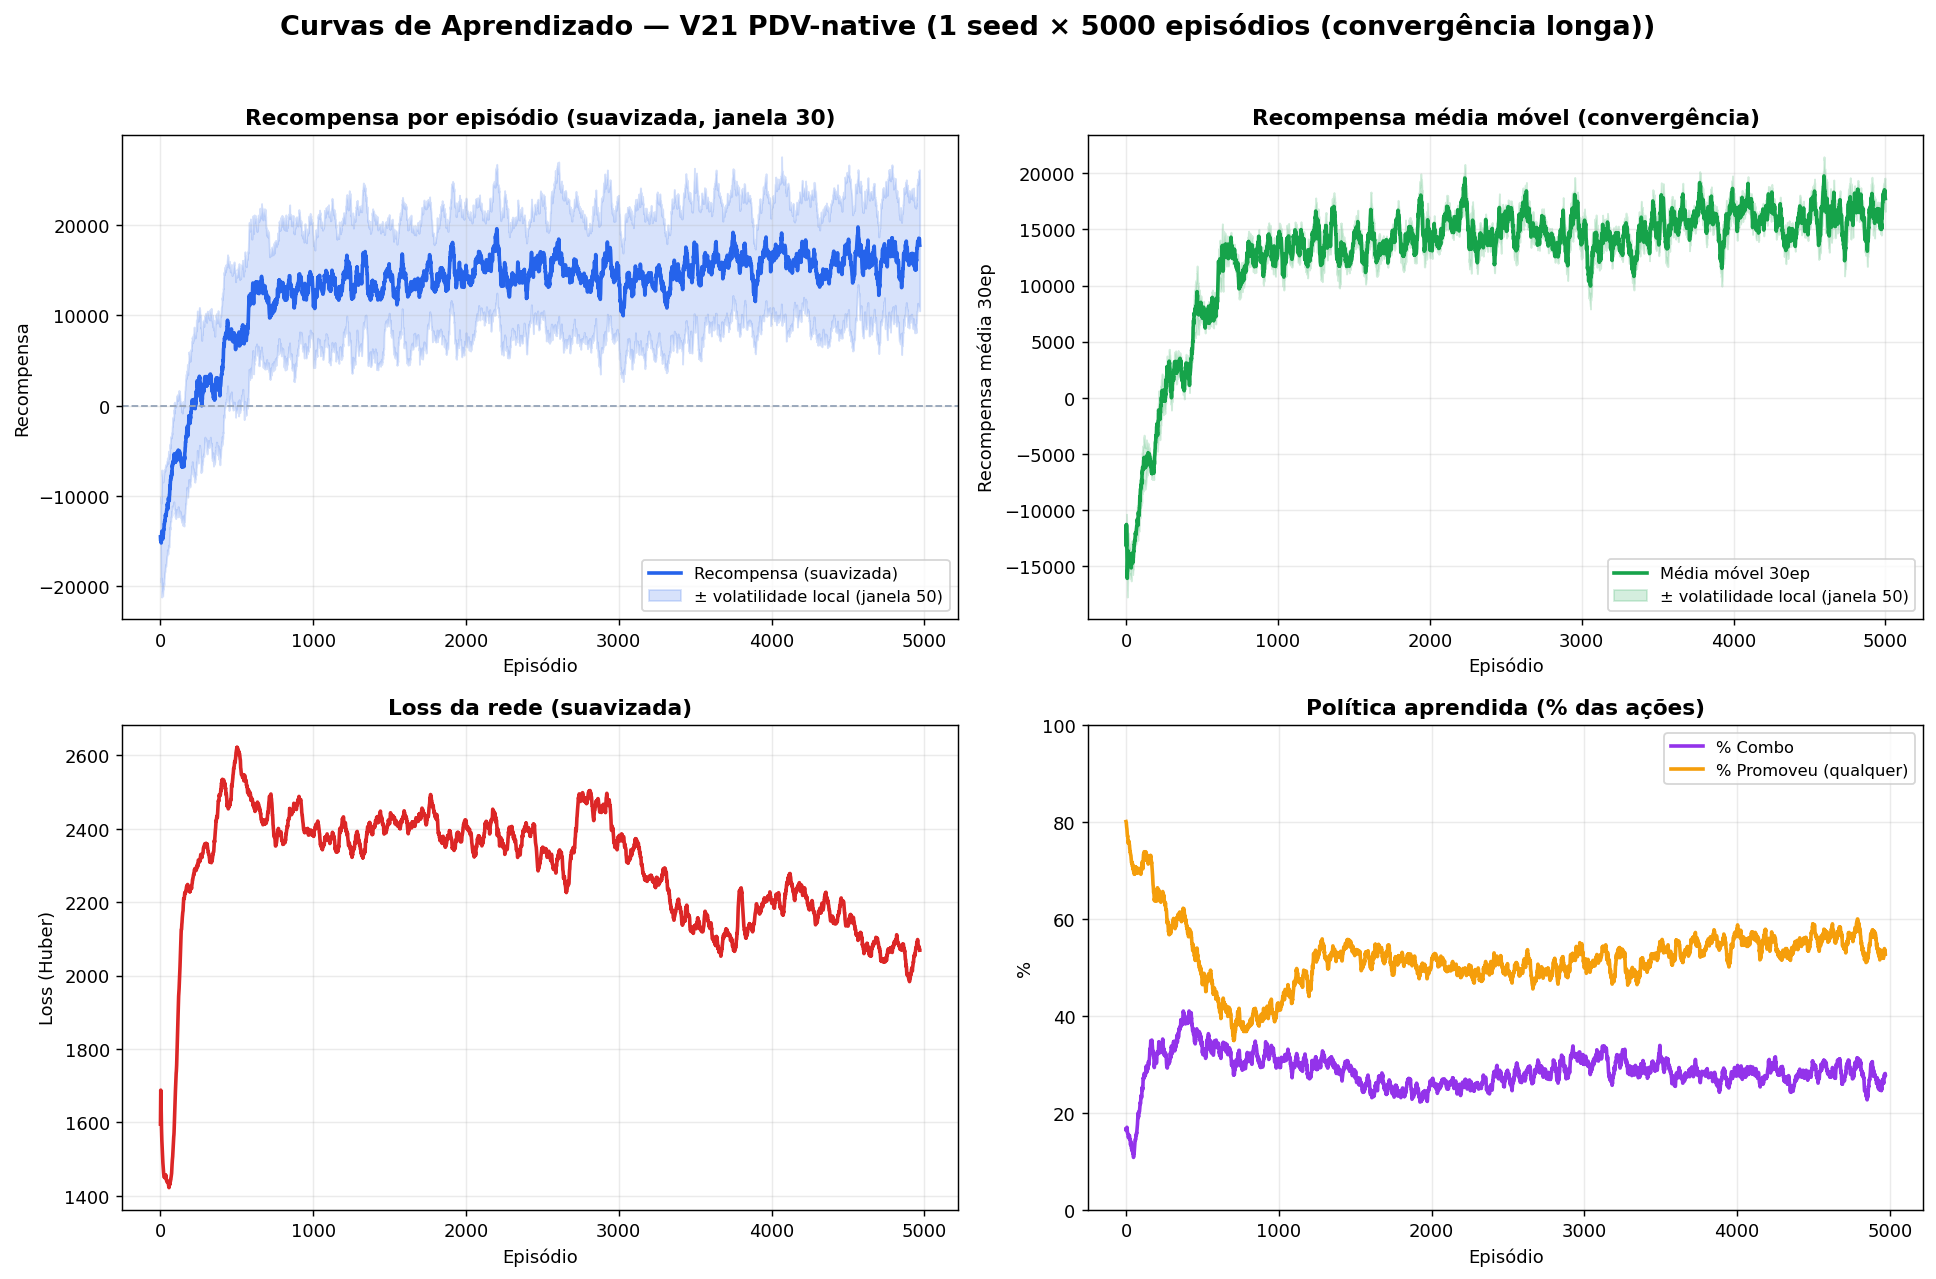
\includegraphics[width=\columnwidth]{Figures/curvas_treino.png}
       \caption{Curvas de aprendizado (1 \textit{seed} $\times$ 5000
       episódios): recompensa por episódio com volatilidade local, média
       móvel, \textit{loss} da rede e política aprendida (\% de combo e
       de promoção).}
   \label{fig:curvas}
\end{figure}

Na validação determinística (rollout de 365 dias), o agente acerta
\textbf{\(11/12\) cenários canônicos de \textit{sanity}} e gera um
calendário anual de \(208\) campanhas (88 combos + 120 descontos
diretos) com \textbf{zero combos inválidos para posto} --- aprendeu a
regra de domínio sem que ela fosse imposta na inferência --- e lucro
adicional estimado de \textbf{R\$ 16.918/ano}.

\textbf{Combos que o agente descobriu.} Os padrões emergiram da
recompensa, não de regras fixas, e fazem sentido de varejo: a
\textbf{``Esquenta de Sexta''} (cerveja + salgadinho em sex/sáb) é o
combo nº 1 do ano (\(\sim45\) ocorrências); \textbf{café + padaria}
domina a manhã de quem para no posto a caminho do trabalho;
\textbf{Chocolate (caixa)} entra como presente nas datas comerciais
(Mães, Namorados, Pais, Crianças); e nos jogos do Brasil na Copa o
agente sobe \textbf{cerveja + petisco} (12 jogos cobertos).

\textbf{Casos difíceis que ele acertou.} O valor do modelo aparece onde
a decisão é sutil: (i) acerta as \textbf{datas-presente} (Dia das Mães,
Namorados) --- justamente onde versões anteriores falhavam por completo
(F1\(=0\) no V11), pois o sinal histórico desses produtos é raro;
(ii) \textbf{recusa combos de supermercado} (gelo + whisky) mesmo quando
o evento ``puxaria'' o combo --- distinção fina de contexto de balcão
aprendida sem regra rígida; (iii) \textbf{protege margem}: não dá
desconto em produto que já está em alta natural, mas desconta produto de
baixo giro para girar estoque --- uma regra de varejo não-trivial que
emergiu sozinha.

\textbf{Entrega para o dono.} O pipeline gera automaticamente um
\textbf{calendário visual em HTML} (Figura~\ref{fig:calendario}): os 12
meses do ano, cada dia colorido por tipo de campanha (Esquenta de Sexta,
jogo da Copa, data comercial, combo, desconto direto), com os destaques
do plano e o lucro adicional estimado (R\$ 16.918/ano; 88 combos e 120
descontos diretos). É o produto final --- um plano que o dono imprime e
segue, com a justificativa de cada campanha.

\begin{figure}[htbp]
   \centering
       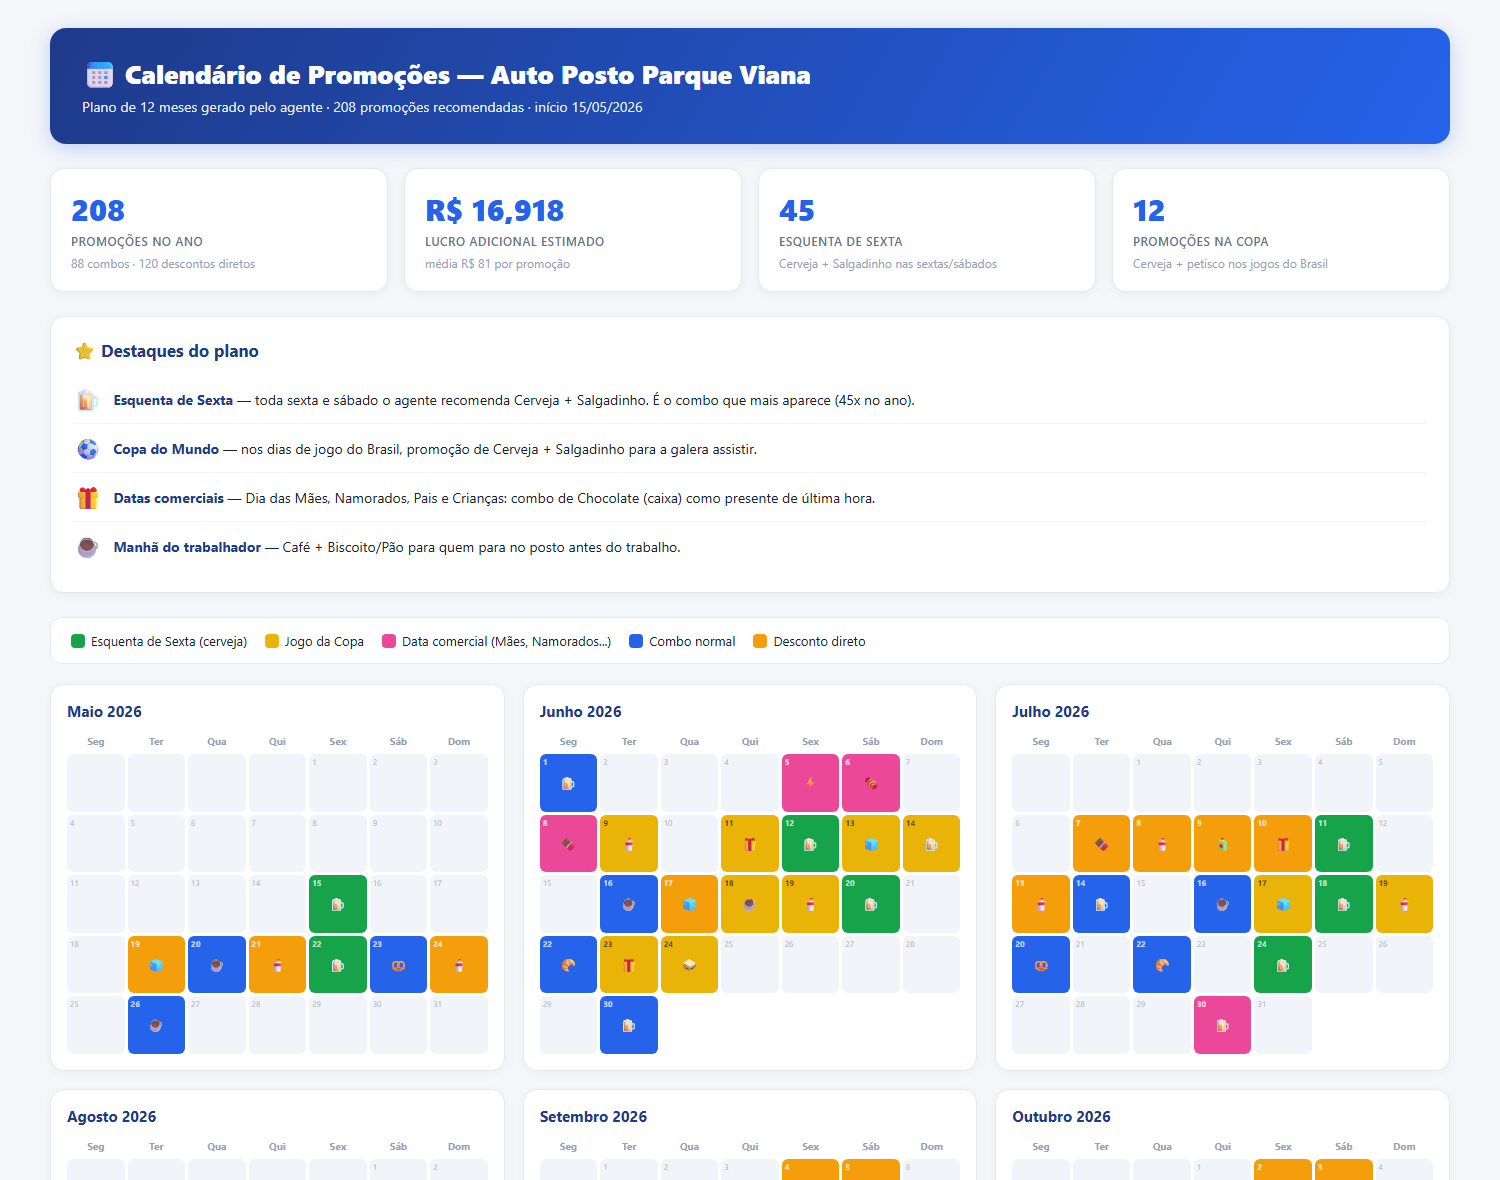
\includegraphics[width=\columnwidth]{Figures/calendario_visual.png}
       \caption{Entregável operacional: calendário visual gerado
       automaticamente pelo agente --- indicadores do ano, destaques do
       plano e os 12 meses com cada campanha codificada por cor.}
   \label{fig:calendario}
\end{figure}

\section{Considerações finais}

\taustart{O} objetivo --- um agente que decide promoções para maximizar
lucro e reduzir vencimento --- foi atingido em termos metodológicos: o
\textit{Branching Double DQN} converge de forma estável, produz um
calendário operacional íntegro (zero combos inválidos) e faz emergir
estratégias de varejo plausíveis sem programá-las explicitamente.

A \textbf{limitação central, assumida abertamente}, é de
\textit{off-policy evaluation}: o ambiente foi calibrado com seis anos de
vendas \textit{sem promoção} e a elasticidade promocional vem da
literatura \cite{bijmolt2005}, não medida no posto. Portanto os valores em
R\$ são \textbf{estimativas de simulação}, não medições. Além disso, as
decisões do agente são fortemente \textit{induzidas} pelo
\textit{reward shaping}, pelo pré-treino e pelo \textit{curriculum} --- o
que genuinamente emerge é o \textit{timing}, a combinação e a quantidade,
não a noção de harmonia em si. O próximo passo necessário é um teste
A/B in loco (semanas com e sem o agente) para calibrar a elasticidade
real e fechar o ciclo de validação. A contribuição do trabalho é o
\textbf{método reprodutível e a honestidade calibrada} sobre o que está e
o que não está validado por dados.

\addcontentsline{toc}{section}{Referências}
\printbibliography

\end{document}
